\section{Udviklingsmetoder}

\subsection{Agil udvikling}
Agil betyder forandringsparathed.
Centrale værdier for agil softwareudvikling.

Individer og interaktioner er vigigere end processer og værktøjer. Software, der virker, er vigtigere end omfattende dokumentation.
Samarbejde med kunden er vigtigere end kontraktforhandling. At kunne reagere på forandringer er vigtigere end at følge en plan.


\textbf{The agile enterprise}
\begin{itemize}
	\item{Der skal være en stærk virksomhedsideologi}
	\item{Der skal være en stærk virksomhedskultur med afsæt i ideologien.}
	\item{Man skal kunne agere proaktivt.}
	\item{Man skal kunne reagere reaktivt.The agile enterprise}
	\item{Forandringsparathed skal kunne måles}
	\item{Virksomheden skal råde over en række genbrugelige komponenter, som nemt kan kombineres.}
	\item{Ovennævnte plug-in kompatibilitet understøttes aktivt af udviklende standarder.}
	\item{Medarbejderne skal kunne eksperimentere frit i selvorganiserende grupper}
	\item{Virksomheden skal facilitere videndeling.}
	\item {Koordinering finder sted på individniveau}
\end{itemize}

\subsection{Kanban}
Kanban er en metode til at styre flowet af arbejdet. Man bruger "noter" på "tavler" til at visualisere og holde styr på projektet.

\begin{center}
	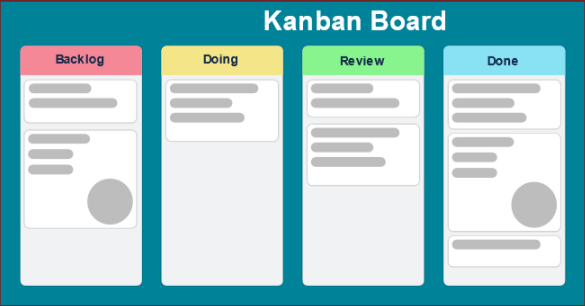
\includegraphics[width=0.8\textwidth]{Images/Kanban.png}
\end{center}

Ved Kanban har man et commitment point, hvor vi beslutter os for at det skal udføres.
Dertil er der lead time, som er hvor lang tid det tager at gennemføre. En vigtig begrænsing er  WIP limits.
Work in progress limits sikrer at man færdiggører opgaver og ikke bare tilføjer flere.


\subsection{Rubber duck debugging}
Ved at forklare sit problem kan man bedre forstå det.

\subsection{Extreme programming}
Vi prøver ikke at at forudse alt hvad der skal laves. I stedet fokuseres
der på det mest værdifulde og så starter vi der. Da der ikke er lavet
overordnede planer er der stor risiko for kaos. Der er derfor oprettet
forskellige regler for at holde styr på kaosset. Det gøres ved forskellige
niveauer af feedback.

\textbf{Pair programming}

I extreme programming programmerer man ikke alene. Man gør det altid i par.
Den ene skriver kode og arbejder med at finde den umiddelbare løsning.
Den anden er "navigatør/observatør" og laver review af koden og er
opmærksom på den længeresigtede planlægning.

\textbf{Stand-up meetings}

Man mødes alle på holdet først om dagen. Mødet foregår stående så det
ikke tager for lang tid. Man fortæller hvad man er i gang med at arbejde på
og om der er problemer. Derved ved hele holdet hvor alle er og muligheder
for samarbejde forbedres.

\textbf{Acceptance tests}
Er det vi har lavet acceptabelt for kunden? Der laves tests for kunden
der viser det nuværende system. Eventuelle uoverensstemmelser kan rettes
hurtigt i projektet.


\begin{center}
	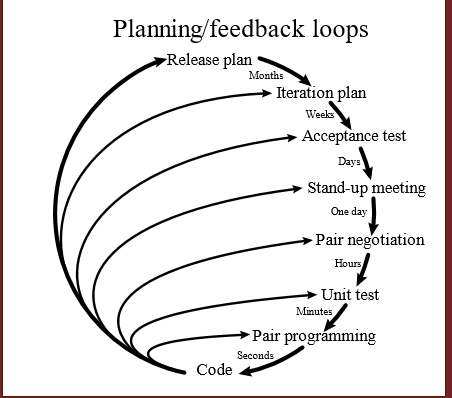
\includegraphics[width=0.7\textwidth]{Images/extreme.png}
\end{center}


\subsection{Vandfaldsmodellen}
Vi prøver at planlægge det hele fra starten af. Der kan være mange
grunde til at vi ikke når i mål, og så står vi pludseligt uden
nogen som helst værdi.

\begin{center}
	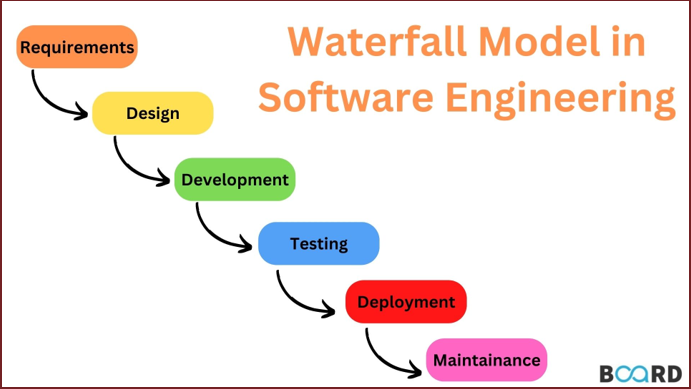
\includegraphics[width=0.7\textwidth]{Images/vandfald.png}
\end{center}
